\documentclass[tikz,border=6pt]{standalone}
\usetikzlibrary{arrows.meta,positioning,calc,backgrounds}
\tikzset{
  every node/.style={font=\sffamily},
  compute/.style={draw=orange!70!black, fill=orange!40, rounded corners=2pt, line width=0.6pt, align=center, inner sep=3.5pt},
  computefz/.style={compute, dashed},
  feature/.style={draw=blue!45!black, fill=blue!12, rounded corners=2pt, line width=0.6pt, align=center, inner sep=3.5pt},
  stepbox/.style={draw=orange!55!black, fill=yellow!14, rounded corners=2pt, line width=0.5pt, align=center, inner sep=3pt},
  headbox/.style={draw=blue!45!black, fill=blue!16, rounded corners=2pt, line width=0.6pt, align=center, inner sep=3.5pt},
  outbox/.style={draw=green!45!black, fill=green!10, rounded corners=2pt, line width=0.7pt, align=center, inner sep=3.5pt},
  flow/.style={-{Stealth[length=5pt,width=4pt]}, line width=0.75pt, draw=black!75},
  flowd/.style={flow, dashed},
  flowg/.style={-{Stealth[length=5pt,width=4pt]}, line width=0.9pt, draw=green!45!black},
  lab/.style={font=\sffamily\tiny, text=black!60, inner sep=1pt, align=center},
  labg/.style={font=\sffamily\tiny\bfseries, text=green!35!black, inner sep=1pt},
  plus/.style={circle, draw=green!45!black, fill=green!12, line width=0.8pt, inner sep=1.0pt, font=\sffamily\scriptsize\bfseries},
  panel/.style={draw=black!55, dashed, rounded corners=9pt, line width=0.7pt, fill=white},
  tab/.style={rounded corners=2pt, inner sep=2.5pt, font=\sffamily\scriptsize\bfseries, text=white},
  ttl/.style={font=\sffamily\scriptsize\bfseries},
  sub/.style={font=\sffamily\tiny, text=black!70},
  plane/.style={fill=blue!18, draw=orange!80!black, line width=0.55pt},
}
\def\ttl{\sffamily\scriptsize\bfseries}
\def\subf{\sffamily\tiny}
\begin{document}
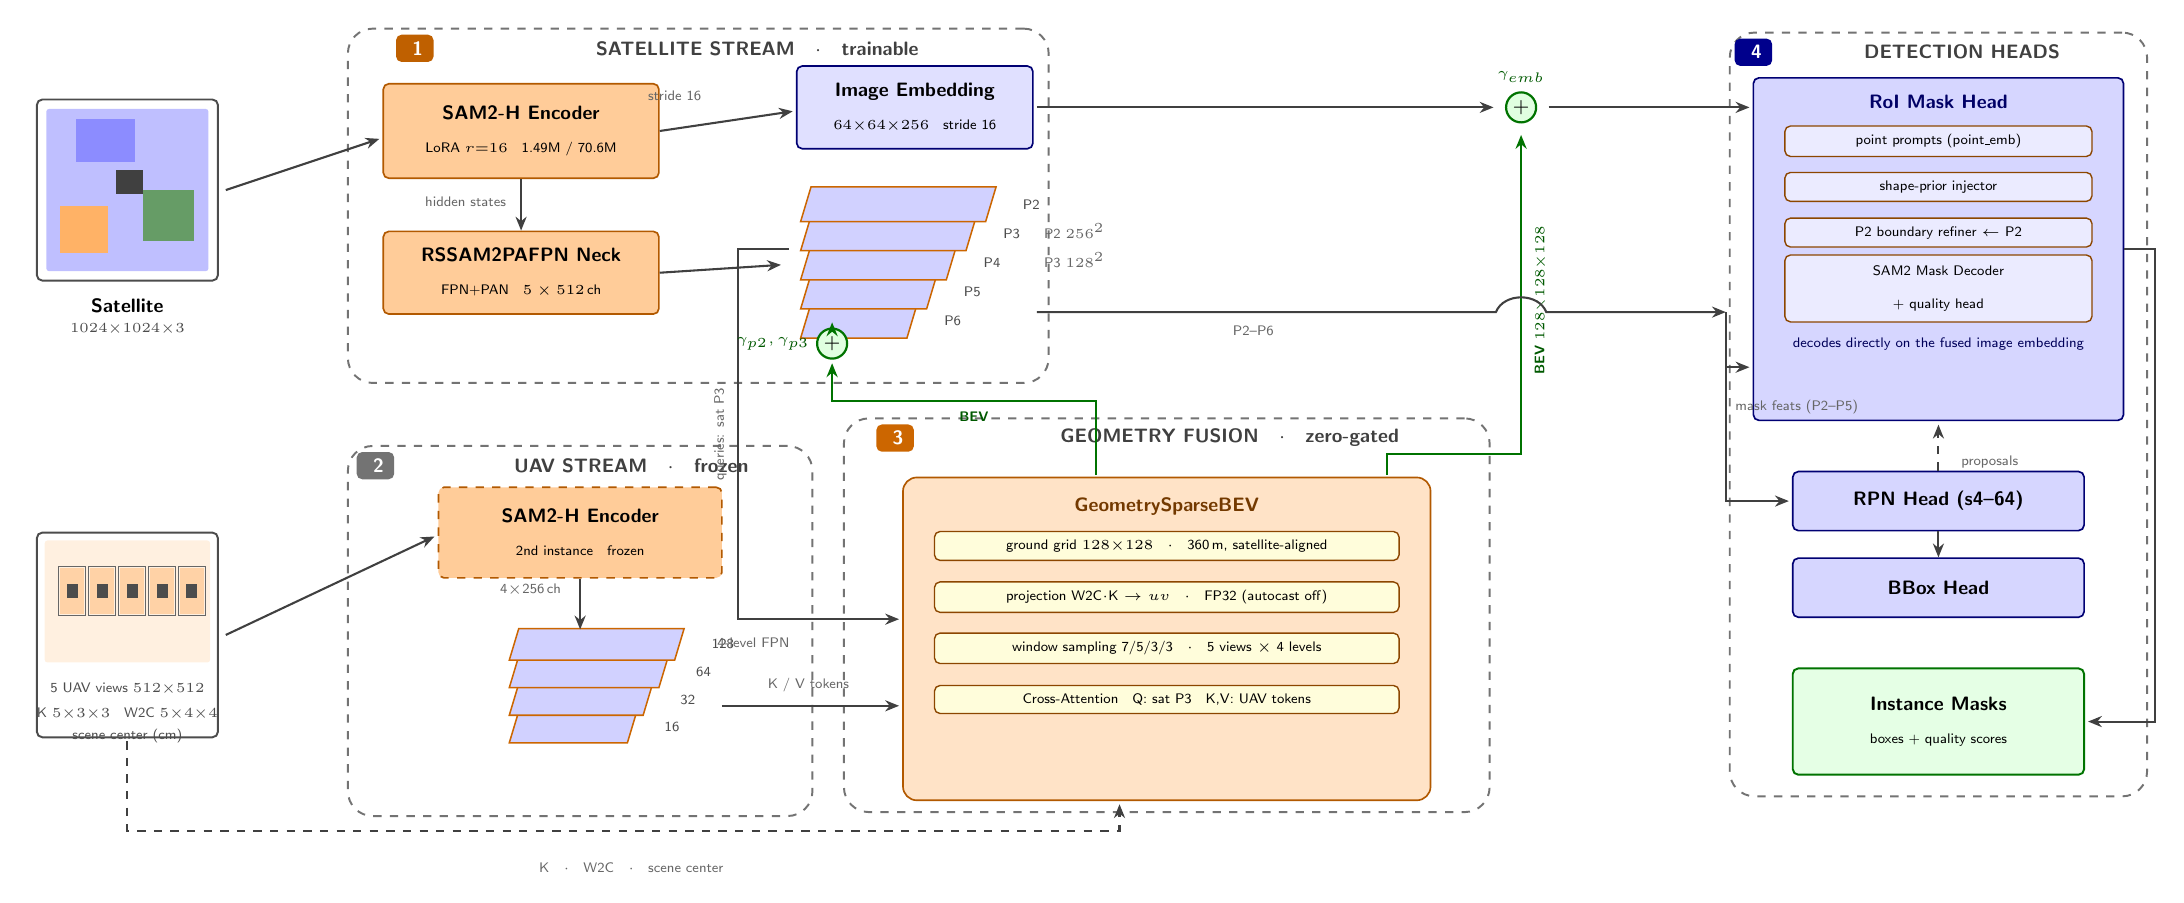
\begin{tikzpicture}[x=1cm,y=1cm]

% ================= INPUT THUMBNAILS =================
\begin{scope}[shift={(0.45,7.15)}]
  \draw[draw=black!70, line width=0.7pt, rounded corners=2pt] (0,0) rectangle (2.3,2.3);
  \fill[blue!25, rounded corners=1pt] (0.12,0.12) rectangle (2.18,2.18);
  \fill[blue!45] (0.5,1.5) rectangle (1.25,2.05);
  \fill[green!35!black!60] (1.35,0.5) rectangle (2.0,1.15);
  \fill[orange!60] (0.3,0.35) rectangle (0.9,0.95);
  \fill[black!75] (1.0,1.1) rectangle (1.35,1.4);
  \node[ttl] at (1.15,-0.32) {Satellite};
  \node[sub] at (1.15,-0.62) {$1024{\times}1024{\times}3$};
\end{scope}

\begin{scope}[shift={(0.45,1.35)}]
  \draw[draw=black!70, line width=0.7pt, rounded corners=2pt] (0,0) rectangle (2.3,2.6);
  \fill[orange!12, rounded corners=1pt] (0.1,0.95) rectangle (2.2,2.5);
  \foreach \i in {0,...,4} {
    \begin{scope}[shift={(0.28+0.38*\i,1.55)}]
      \draw[draw=black!60, line width=0.4pt] (0,0) rectangle (0.34,0.62);
      \fill[orange!35] (0.02,0.02) rectangle (0.32,0.6);
      \fill[black!70] (0.1,0.22) rectangle (0.24,0.4);
    \end{scope}}
  \node[sub] at (1.15,0.62) {5 UAV views $512{\times}512$};
  \node[sub] at (1.15,0.3) {K $5{\times}3{\times}3$ \; W2C $5{\times}4{\times}4$};
  \node[sub] at (1.15,0.02) {scene center (cm)};
\end{scope}

% ================= PANEL 1 : SATELLITE STREAM =================
\node[panel, minimum width=8.9cm, minimum height=4.5cm] at (8.85,8.1) {};
\node[tab, fill=orange!75!black] at (5.25,10.1) {\,\;1\,};
\node[ttl, text=black!75] at (9.6,10.1) {SATELLITE STREAM \; $\cdot$ \; trainable};

\node[compute, minimum width=3.5cm, minimum height=1.2cm] (enc) at (6.6,9.05)
  {{\ttl SAM2-H Encoder}\\{\subf LoRA $r{=}16$ \; 1.49M / 70.6M}};
\node[feature, minimum width=3.0cm, minimum height=1.05cm] (imgemb) at (11.6,9.35)
  {{\ttl Image Embedding}\\{\subf $64{\times}64{\times}256$ \; stride 16}};
\node[compute, minimum width=3.5cm, minimum height=1.05cm] (neck) at (6.6,7.25)
  {{\ttl RSSAM2PAFPN Neck}\\{\subf FPN+PAN \; $5\times512$\,ch}};

% FPN pyramid: stacked isometric planes
\foreach \i/\name/\pw in {0/P6/1.35,1/P5/1.6,2/P4/1.85,3/P3/2.1,4/P2/2.35} {
  \begin{scope}[shift={(10.15,6.42+0.37*\i)}, xslant=0.30]
    \draw[plane] (0,0) rectangle (\pw,0.44);
  \end{scope}
  \node[sub, anchor=west] at ($(10.15+\pw+0.35, 6.64+0.37*\i)$) {\name};
}
\node[lab, anchor=west] at (13.2,7.78) {P2 $256^2$};
\node[lab, anchor=west] at (13.2,7.41) {P3 $128^2$};

% ================= PANEL 2 : UAV STREAM =================
\node[panel, minimum width=5.9cm, minimum height=4.7cm] at (7.35,2.7) {};
\node[tab, fill=black!55] at (4.75,4.8) {\,\;2\,};
\node[ttl, text=black!75] at (8.0,4.8) {UAV STREAM \; $\cdot$ \; frozen};

\node[computefz, minimum width=3.6cm, minimum height=1.15cm] (denc) at (7.35,3.95)
  {{\ttl SAM2-H Encoder}\\{\subf 2nd instance \; frozen}};
\foreach \i/\name/\pw in {0/16/1.5,1/32/1.7,2/64/1.9,3/128/2.1} {
  \begin{scope}[shift={(6.45,1.28+0.35*\i)}, xslant=0.30]
    \draw[plane] (0,0) rectangle (\pw,0.4);
  \end{scope}
  \node[sub, anchor=west] at ($(6.45+\pw+0.35, 1.48+0.35*\i)$) {\name};
}
\node[lab, anchor=west] at (9.05,2.55) {4-level FPN};

% ================= PANEL 3 : GEOMETRY FUSION =================
\node[panel, minimum width=8.2cm, minimum height=5.0cm] at (14.8,2.9) {};
\node[tab, fill=orange!80!black] at (11.35,5.15) {\,\;3\,};
\node[ttl, text=black!75] at (15.6,5.15) {GEOMETRY FUSION \; $\cdot$ \; zero-gated};

\node[compute, rounded corners=5pt, fill=orange!22, minimum width=6.7cm, minimum height=4.1cm] (bevbox) at (14.8,2.6) {};
\node[ttl, text=orange!45!black] at (14.8,4.28) {GeometrySparseBEV};
\node[stepbox, minimum width=5.9cm] at (14.8,3.78) {{\subf ground grid $128{\times}128$ \; $\cdot$ \; 360\,m, satellite-aligned}};
\node[stepbox, minimum width=5.9cm] at (14.8,3.13) {{\subf projection W2C$\cdot$K $\to uv$ \; $\cdot$ \; FP32 (autocast off)}};
\node[stepbox, minimum width=5.9cm] at (14.8,2.48) {{\subf window sampling 7/5/3/3 \; $\cdot$ \; 5 views $\times$ 4 levels}};
\node[stepbox, minimum width=5.9cm] at (14.8,1.83) {{\subf Cross-Attention \; Q: sat P3 \; K,V: UAV tokens}};

% ================= PANEL 4 : DETECTION HEADS =================
\node[panel, minimum width=5.3cm, minimum height=9.7cm] at (24.6,5.45) {};
\node[tab, fill=blue!55!black] at (22.25,10.05) {\,\;4\,};
\node[ttl, text=black!75] at (24.9,10.05) {DETECTION HEADS};

\node[headbox, minimum width=4.7cm, minimum height=4.35cm] (mhbox) at (24.6,7.55) {};
\node[ttl, text=blue!40!black] at (24.6,9.42) {RoI Mask Head};
\node[stepbox, fill=blue!8, minimum width=3.9cm] at (24.6,8.92) {{\subf point prompts (point\textunderscore emb)}};
\node[stepbox, fill=blue!8, minimum width=3.9cm] at (24.6,8.34) {{\subf shape-prior injector}};
\node[stepbox, fill=blue!8, minimum width=3.9cm] at (24.6,7.76) {{\subf P2 boundary refiner $\leftarrow$ P2}};
\node[stepbox, fill=blue!8, minimum width=3.9cm, minimum height=0.85cm] at (24.6,7.05) {{\subf SAM2 Mask Decoder}\\{\subf + quality head}};
\node[lab, text=blue!35!black] at (24.6,6.35) {decodes directly on the fused image embedding};

\node[headbox, minimum width=3.7cm, minimum height=0.75cm] (rpn) at (24.6,4.35) {{\ttl RPN Head (s4--64)}};
\node[headbox, minimum width=3.7cm, minimum height=0.75cm] (bboxh) at (24.6,3.25) {{\ttl BBox Head}};
\node[outbox, minimum width=3.7cm, minimum height=1.35cm] (out) at (24.6,1.55)
  {{\ttl Instance Masks}\\{\subf boxes + quality scores}};

% ================= ARROWS =================
\draw[flow] (2.85,8.3) -- (4.8,8.95);
\draw[flow] (enc.south) -- (neck.north);
\node[lab, anchor=east] at (6.45,8.15) {hidden states};
\draw[flow] (enc.east) -- (10.05,9.3);
\node[lab] at (8.55,9.5) {stride 16};
\draw[flow] (neck.east) -- (9.9,7.35);

\draw[flow] (2.85,2.65) -- (5.5,3.9);
\draw[flow] (denc.south) -- (7.35,2.72);
\node[lab, anchor=east] at (7.15,3.22) {4$\times$256\,ch};

% K/V tokens: UAV FPN -> BEV
\draw[flow] (9.15,1.75) -- (11.4,1.75);
\node[lab] at (10.25,2.02) {K / V tokens};
% calibration: UAV input -> BEV (below panels)
\draw[flowd] (1.6,1.3) -- (1.6,0.16) -- (14.2,0.16) -- (14.2,0.5);
\node[lab, text=black!60] at (8.0,-0.3) {K \; $\cdot$ \; W2C \; $\cdot$ \; scene center};
% queries: P3 plane -> BEV west
\draw[flow] (10.0,7.55) -- (9.35,7.55) -- (9.35,2.85) -- (11.4,2.85);
\node[lab, rotate=90] at (9.13,5.2) {queries: sat P3};

% BEV -> P2/P3 gate (up through corridor)
\node[labg] at (12.35,5.42) {BEV};
\draw[flowg] (13.9,4.68) -- (13.9,5.62) -- (10.55,5.62) -- (10.55,6.1);
\node[plus] (p2p3) at (10.55,6.35) {$+$};
\draw[flowg] (p2p3.north) -- (10.55,6.62);
\node[labg, anchor=east] at (10.3,6.35) {$\gamma_{p2},\gamma_{p3}$};

% BEV -> embedding gate (riser on the right)
\draw[flowg] (17.6,4.68) -- (17.6,4.95) -- (19.3,4.95) -- (19.3,9.0);
\node[labg, rotate=90] at (19.55,6.9) {BEV $128{\times}128{\times}128$};

% image embedding -> plus -> mask head
\node[plus] (pemb) at (19.3,9.35) {$+$};
\draw[flow] (13.15,9.35) -- (18.95,9.35);
\node[labg, anchor=south] at (19.3,9.62) {$\gamma_{emb}$};
\draw[flow] (19.65,9.35) -- (22.2,9.35);

% trunk pyramid -> heads, with hop over the riser
\draw[flow] (13.15,6.75) -- (18.98,6.75) .. controls (19.08,7.0) and (19.52,7.0) .. (19.62,6.75) -- (21.9,6.75);
\node[lab] at (15.9,6.52) {P2--P6};
\draw[flow] (21.9,6.75) -- (21.9,4.35) -- (22.7,4.35);
\draw[flow] (21.9,6.75) -- (21.9,6.05) -- (22.2,6.05);
\node[lab, anchor=west] at (21.98,5.55) {mask feats (P2--P5)};

\draw[flow] (rpn.south) -- (bboxh.north);
\draw[flowd] (rpn.north) -- (24.6,5.32);
\node[lab, anchor=west] at (24.85,4.85) {proposals};
\draw[flow] (mhbox.east) -- (27.35,7.55) -- (27.35,1.55) -- (26.5,1.55);

\end{tikzpicture}
\end{document}
